\documentclass[10.5pt,a4paper]{article}
\usepackage[margin=1.45cm]{geometry}
\usepackage{amsmath,amssymb,mathtools}
\usepackage{booktabs,array,longtable,tabularx,multirow}
\usepackage{tikz}
\usetikzlibrary{arrows.meta,positioning,calc,shapes.geometric}
\usepackage[most]{tcolorbox}
\usepackage{xcolor}
\usepackage{enumitem}
\usepackage{fancyhdr}
\usepackage{microtype}
\usepackage[T1]{fontenc}
\usepackage{lmodern}
\usepackage{hyperref}
\hypersetup{hidelinks}

\definecolor{primary}{HTML}{1F4E78}
\definecolor{qblue}{HTML}{EAF3FF}
\definecolor{ablue}{HTML}{EEF9F0}
\definecolor{qborder}{HTML}{2E75B6}
\definecolor{aborder}{HTML}{2E8B57}
\definecolor{noteorange}{HTML}{FFF4E5}
\definecolor{orangeborder}{HTML}{D98200}
\definecolor{deep}{HTML}{17365D}
\definecolor{graybox}{HTML}{F6F7F9}

\pagestyle{fancy}
\fancyhf{}
\lhead{CSE-3203: Design and Analysis of Algorithms-II}
\rhead{Final 2021 - Complete Q\&A Notes}
\cfoot{\thepage}
\setlength{\headheight}{14pt}

\newtcolorbox{questionbox}[2][]{
  enhanced, breakable,
  colback=qblue, colframe=qborder,
  boxrule=0.9pt, arc=1.5mm,
  title={\textbf{#2}}, fonttitle=\bfseries,
  coltitle=white, colbacktitle=qborder,
  attach boxed title to top left={xshift=2mm,yshift=-2mm},
  boxed title style={arc=1mm,boxrule=0pt},
  before skip=8pt, after skip=5pt,#1
}
\newtcolorbox{answerbox}[1][]{
  enhanced, breakable,
  colback=ablue, colframe=aborder,
  boxrule=0.8pt, arc=1.5mm,
  title={\textbf{Answer}}, fonttitle=\bfseries,
  coltitle=white, colbacktitle=aborder,
  attach boxed title to top left={xshift=2mm,yshift=-2mm},
  boxed title style={arc=1mm,boxrule=0pt},
  before skip=4pt, after skip=9pt,#1
}
\newtcolorbox{examtip}[1][]{
  enhanced, breakable,colback=noteorange,colframe=orangeborder,
  title={\textbf{Exam Tip}},fonttitle=\bfseries,coltitle=white,colbacktitle=orangeborder,
  boxrule=0.7pt,arc=1mm,#1
}
\newtcolorbox{keybox}[1][]{
  enhanced, breakable,colback=graybox,colframe=deep,
  title={\textbf{Key Result}},fonttitle=\bfseries,coltitle=white,colbacktitle=deep,
  boxrule=0.7pt,arc=1mm,#1
}

\newcommand{\Oh}{\mathcal{O}}
\newcommand{\Th}{\Theta}
\newcommand{\floor}[1]{\left\lfloor #1\right\rfloor}
\newcommand{\ceil}[1]{\left\lceil #1\right\rceil}

\begin{document}

\begin{center}
{\LARGE\bfseries\color{primary} CSE-3203 Final Examination 2021}\par
\vspace{2mm}
{\Large\bfseries Design and Analysis of Algorithms-II}\par
\vspace{1mm}
{\large Complete Question \& Answer Notes}\par
\vspace{3mm}
\rule{0.9\textwidth}{0.6pt}
\end{center}

\begin{examtip}
The questions below are transcribed from the two supplied exam-page screenshots. The solutions are worked study notes. For questions whose wording is slightly ambiguous, the interpretation used is stated explicitly.
\end{examtip}

\tableofcontents
\newpage

% ---------------- Q1 ----------------
\section{Question 1 - Hashing}

\begin{questionbox}{Q1(a) [6 marks]}
Insert the keys
\[
10,22,31,4,15,28,17,88,59
\]
into a hash table of length \(m=11\) using double hashing with
\[
h_1(k)=k,\qquad h_2(k)=1+(k\bmod (m-1)).
\]
\end{questionbox}

\begin{answerbox}
For double hashing we use
\[
h(k,i)=\bigl(h_1(k)+i\,h_2(k)\bigr)\bmod m,
\]
so effectively \(h_1(k)\bmod 11\) gives the initial slot.

\begin{center}
\small
\begin{tabular}{c c c l c}
\toprule
Key & \(h_1(k)\bmod11\) & \(h_2(k)\) & Probe sequence & Final slot\\
\midrule
10 & 10 & 1  & 10 & 10\\
22 & 0  & 3  & 0 & 0\\
31 & 9  & 2  & 9 & 9\\
4  & 4  & 5  & 4 & 4\\
15 & 4  & 6  & 4,10,5 & 5\\
28 & 6  & 9  & 6 & 6\\
17 & 6  & 8  & 6,3 & 3\\
88 & 0  & 9  & 0,9,7 & 7\\
59 & 4  & 10 & 4,3,2 & 2\\
\bottomrule
\end{tabular}
\end{center}

Final table:
\[
\begin{array}{c|ccccccccccc}
\text{Index} &0&1&2&3&4&5&6&7&8&9&10\\ \hline
\text{Key} &22&-&59&17&4&15&28&88&-&31&10
\end{array}
\]
\end{answerbox}

\begin{questionbox}{Q1(b) [4 marks]}
After completing the insertions of Q1(a), a successful search for a key in the table is claimed to give a verdict within 4 probes on average. Do you agree? Explain.
\end{questionbox}

\begin{answerbox}
For the \emph{inserted keys}, the successful-search probe counts are exactly the same as the insertion probe counts:
\[
1,1,1,1,3,1,2,3,3.
\]
Hence
\[
\text{average probes}=\frac{1+1+1+1+3+1+2+3+3}{9}
=\frac{16}{9}\approx1.78<4.
\]
In fact, every inserted key is found within at most 3 probes.

Therefore, under the natural interpretation ``searching for any key \emph{in the hash table}'' = successful search, the statement is \textbf{true}.

\begin{examtip}
If the statement were meant to include arbitrary unsuccessful searches, the result would not follow from this calculation. At load factor \(\alpha=9/11\), unsuccessful searches can take more probes.
\end{examtip}
\end{answerbox}

\begin{questionbox}{Q1(c) [4 marks]}
Prove that in a hash table in which collisions are resolved by chaining, a successful search takes average-case time \(\Theta(1+\alpha)\) under simple uniform hashing.
\end{questionbox}

\begin{answerbox}
Let \(n\) keys be stored in \(m\) slots and let
\[
\alpha=\frac{n}{m}
\]
be the load factor.

Under simple uniform hashing, each key is equally likely to be hashed to any slot. Therefore the expected chain length is \(\alpha\).

For a successful search, suppose we search for a uniformly chosen stored key. We first compute its hash value in \(\Theta(1)\) time. Inside the chain, the expected number of elements examined is proportional to the expected chain length. More precisely, with insertion at the head, the expected number examined is about
\[
1+\frac{\alpha}{2},
\]
up to constant terms. Hence
\[
E[T_{\text{successful}}]=\Theta(1+\alpha).
\]

\begin{keybox}
\[
\boxed{\text{Successful chaining search}=\Theta(1+\alpha)}
\]
\end{keybox}
\end{answerbox}

% ---------------- Q2 ----------------
\section{Question 2 - Computational Geometry}

\begin{questionbox}{Q2(a) [6 marks]}
For the plotted points, find the convex hull using the Graham-Scan algorithm. A step-by-step graphical demonstration is sufficient.
\end{questionbox}

\begin{answerbox}
The points visible in the supplied figure are
\[
\begin{aligned}
&(-7,8),(-4,6),(2,6),(8,6),(-10,4),(-2,2),\\
&(-8,-2),(3,-2),(7,-2),(-9,-5),(0,-6),(8,-7),(6,-10).
\end{aligned}
\]

Choose the lowest point
\[
p_0=(6,-10)
\]
as the pivot. Sort the remaining points by polar angle around \(p_0\). The points \((7,-2)\) and \((8,6)\) lie on the same ray from \(p_0\), so Graham Scan keeps only the farther point \((8,6)\).

The scan removes points whenever the last three stack points fail to make a left turn. The final stack is
\[
\boxed{(6,-10),(8,-7),(8,6),(-7,8),(-10,4),(-9,-5)}.
\]
Thus these six points form the convex hull.

\begin{center}
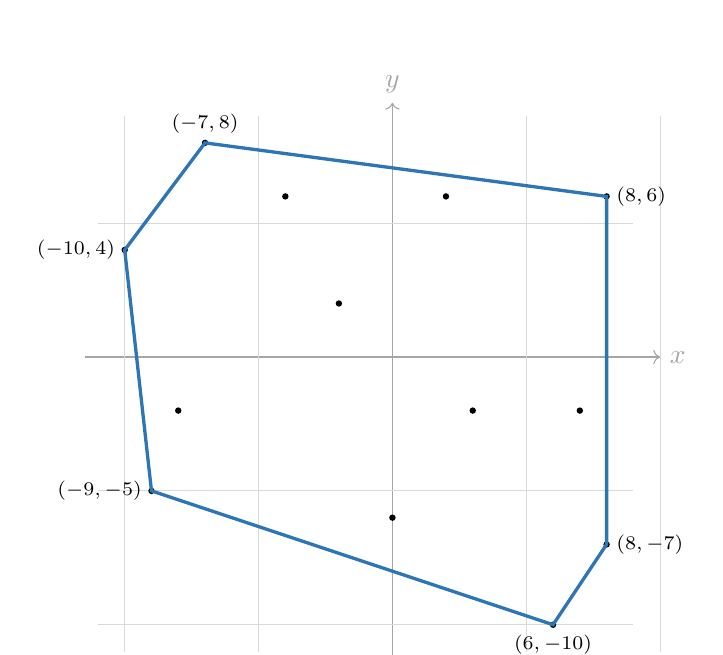
\begin{tikzpicture}[scale=0.34]
  \draw[->,gray!70] (-11.5,0)--(10,0) node[right]{\(x\)};
  \draw[->,gray!70] (0,-11.5)--(0,9.5) node[above]{\(y\)};
  \foreach \x in {-10,-5,5,10} \draw[gray!30] (\x,-11)--(\x,9);
  \foreach \y in {-10,-5,5} \draw[gray!30] (-11,\y)--(9,\y);
  \def\pts{(-7,8),(-4,6),(2,6),(8,6),(-10,4),(-2,2),(-8,-2),(3,-2),(7,-2),(-9,-5),(0,-6),(8,-7),(6,-10)}
  \foreach \p in \pts {\fill[black] \p circle (0.12);}
  \draw[very thick,qborder] (6,-10)--(8,-7)--(8,6)--(-7,8)--(-10,4)--(-9,-5)--cycle;
  \node[below] at (6,-10) {\scriptsize\((6,-10)\)};
  \node[right] at (8,-7) {\scriptsize\((8,-7)\)};
  \node[right] at (8,6) {\scriptsize\((8,6)\)};
  \node[above] at (-7,8) {\scriptsize\((-7,8)\)};
  \node[left] at (-10,4) {\scriptsize\((-10,4)\)};
  \node[left] at (-9,-5) {\scriptsize\((-9,-5)\)};
\end{tikzpicture}
\end{center}
\end{answerbox}

\begin{questionbox}{Q2(b) [4 marks]}
Prove that Kirkpatrick-Seidel's convex-hull algorithm takes \(O(n\lg h)\) time, where \(h\) is the number of hull vertices.
\end{questionbox}

\begin{answerbox}
Kirkpatrick-Seidel is output-sensitive. For one side of the hull it repeatedly:
\begin{enumerate}[leftmargin=6mm]
\item splits the point set by a median \(x\)-coordinate,
\item finds the bridge crossing the median line in linear time,
\item discards points that cannot lie on the hull,
\item recursively constructs the two remaining hull portions.
\end{enumerate}

At any fixed recursion depth, the subproblems contain disjoint subsets of the original points, so the total work over that level is \(O(n)\).

The recursion is balanced with respect to the number of \emph{output hull vertices}: the bridge separates the hull into smaller portions, so the recursion depth is \(O(\lg h)\).

Therefore
\[
T(n,h)=O(n)\times O(\lg h)=\boxed{O(n\lg h)}.
\]
The lower hull is handled similarly, so the total remains \(O(n\lg h)\).
\end{answerbox}

\begin{questionbox}{Q2(c) [4 marks]}
Sketch an \(O(n^2\lg n)\)-time algorithm to identify whether any three points in a set of \(n\) points are collinear.
\end{questionbox}

\begin{answerbox}
For each point \(p_i\), use it as a pivot.
\begin{enumerate}[leftmargin=6mm]
\item Compute the polar angle (or slope) from \(p_i\) to every other point.
\item Sort the other \(n-1\) points by that angle in \(O(n\lg n)\).
\item Scan adjacent entries. If two points \(p_j,p_k\) have the same angle from \(p_i\), then \(p_i,p_j,p_k\) are collinear.
\end{enumerate}
Equivalently, for equal-angle candidates verify
\[
(p_j-p_i)\times(p_k-p_i)=0.
\]
Repeating the \(O(n\lg n)\) procedure for all \(n\) pivots gives
\[
\boxed{O(n^2\lg n)}.
\]
\end{answerbox}

% ---------------- Q3 ----------------
\section{Question 3 - String Matching and Finite Automata}

\begin{questionbox}{Q3(a) [6 marks]}
Calculate the prefix function, showing all steps of KMP, for the pattern
\[
P=\texttt{abbababbba}.
\]
\end{questionbox}

\begin{answerbox}
Using 1-based indexing, \(\pi[q]\) is the length of the longest proper prefix of \(P[1..q]\) that is also a suffix.

\begin{center}
\small
\begin{tabular}{c c c c p{6.2cm}}
\toprule
\(q\) & \(P[q]\) & previous \(k\) & \(\pi[q]\) & Reason\\
\midrule
1 & a & - & 0 & First character\\
2 & b & 0 & 0 & \(b\neq a\)\\
3 & b & 0 & 0 & \(b\neq a\)\\
4 & a & 0 & 1 & \(a=P[1]\)\\
5 & b & 1 & 2 & \(b=P[2]\)\\
6 & a & 2 & 1 & mismatch with \(P[3]=b\); fall back to 0, then \(a=P[1]\)\\
7 & b & 1 & 2 & \(b=P[2]\)\\
8 & b & 2 & 3 & \(b=P[3]\)\\
9 & b & 3 & 0 & mismatch with \(P[4]=a\); fall back to 0; \(b\neq P[1]\)\\
10& a & 0 & 1 & \(a=P[1]\)\\
\bottomrule
\end{tabular}
\end{center}

Hence
\[
\boxed{\pi=[0,0,0,1,2,1,2,3,0,1]}.
\]
\end{answerbox}

\begin{questionbox}{Q3(b) [4 marks]}
Using Rabin-Karp on the text
\[
\texttt{3141592653589793}
\]
in modulo-11 fashion, while searching for pattern \(\texttt{26}\), calculate how many times character-by-character checking is required.
\end{questionbox}

\begin{answerbox}
Pattern length \(m=2\), and
\[
26\bmod11=4.
\]
So character-by-character verification is needed only when a 2-digit text window also has hash 4 modulo 11.

\begin{center}
\small
\begin{tabular}{c c c@{\qquad}c c c}
\toprule
Window & mod 11 & Hit? & Window & mod 11 & Hit?\\
\midrule
31&9& &14&3&\\
41&8& &15&4&Yes\\
59&4&Yes&92&4&Yes\\
26&4&Yes&65&10&\\
53&9& &35&2&\\
58&3& &89&1&\\
97&9& &79&2&\\
93&5& & & &\\
\bottomrule
\end{tabular}
\end{center}

Hash matches occur for
\[
\texttt{15},\texttt{59},\texttt{92},\texttt{26}.
\]
Therefore character-by-character checking is triggered
\[
\boxed{4\text{ times}}.
\]
The first three are spurious hits; \(\texttt{26}\) is the true match.

If the examiner counts individual character comparisons rather than verification events, the total is \(1+1+1+2=5\).
\end{answerbox}

\begin{questionbox}{Q3(c) [4 marks]}
Design a finite automaton that can accept both patterns
\[
P_1=\{a_1,a_2,\ldots,a_n,c_1,c_2,\ldots,c_k,b_1,b_2,\ldots,b_m\}
\]
and
\[
P_2=\{p_1,p_2,\ldots,p_o,c_1,c_2,\ldots,c_k,q_1,q_2,\ldots,q_y\}.
\]
Minimize the number of states.
\end{questionbox}

\begin{answerbox}
A compact NFA can share the common middle block \(C=c_1c_2\cdots c_k\). The start state branches into the two distinct prefixes, the branches merge before \(C\), share the \(C\)-path, split into the two suffixes, and finally merge into one accepting state.

\begin{center}
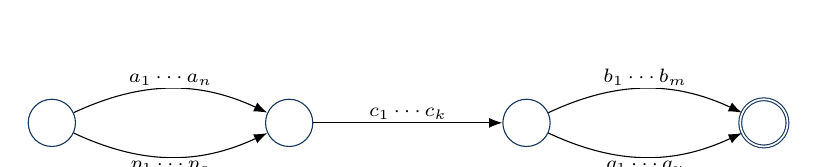
\begin{tikzpicture}[>=Latex,node distance=10mm and 14mm,
  st/.style={circle,draw=deep,minimum size=6mm,inner sep=0pt},
  lab/.style={font=\scriptsize,fill=white,inner sep=1pt}]
\node[st] (s) {};
\node[st, right=24mm of s] (u) {};
\node[st, right=24mm of u] (v) {};
\node[st, double, right=24mm of v] (f) {};
\draw[->] (s) to[bend left=25] node[lab,above] {\(a_1\cdots a_n\)} (u);
\draw[->] (s) to[bend right=25] node[lab,below] {\(p_1\cdots p_o\)} (u);
\draw[->] (u)-- node[lab,above] {\(c_1\cdots c_k\)} (v);
\draw[->] (v) to[bend left=25] node[lab,above] {\(b_1\cdots b_m\)} (f);
\draw[->] (v) to[bend right=25] node[lab,below] {\(q_1\cdots q_y\)} (f);
\end{tikzpicture}
\end{center}

Expanding each multi-symbol label into one transition per symbol, and sharing the start, the common \(C\)-path, the merge/split states, and the final state, gives
\[
\boxed{n+o+k+m+y-1\text{ states}}
\]
for this NFA, assuming no additional accidental equality among the other symbols/substrings. If a total DFA is required, a dead state must also be included, and further minimization depends on equality among the branch symbols.
\end{answerbox}

% ---------------- Q4 ----------------
\section{Question 4 - Backtracking and Permutations}

\begin{questionbox}{Q4(a)(i) [6 marks]}
Write pseudocode to generate distinct permutations of a string containing duplicate characters with time complexity \(O(n^2\cdot n!)\).
\end{questionbox}

\begin{answerbox}
At recursion level \(l\), swap each unused distinct character into position \(l\). Before using \(A[i]\), scan positions \(l..i-1\) to see whether the same character was already used at that level.

\begin{verbatim}
PERMUTE-DISTINCT(A, l, r)
    if l == r
        print A
        return

    for i = l to r
        duplicate = false
        for j = l to i-1
            if A[j] == A[i]
                duplicate = true
                break

        if not duplicate
            swap A[l], A[i]
            PERMUTE-DISTINCT(A, l+1, r)
            swap A[l], A[i]
\end{verbatim}

There are at most \(n!\) leaves. Duplicate checking may cost \(O(n)\) at each recursion step, and a root-to-leaf path has \(O(n)\) levels. Thus the requested loose bound is
\[
\boxed{O(n^2 n!)}.
\]
\end{answerbox}

\begin{questionbox}{Q4(a)(ii) [4 marks]}
Modify the above algorithm to generate all permutations of a string without duplicate characters. Show that its time complexity is \(O(n\cdot n!)\).
\end{questionbox}

\begin{answerbox}
If all characters are distinct, the duplicate test is unnecessary.

\begin{verbatim}
PERMUTE(A, l, r)
    if l == r
        print A
        return

    for i = l to r
        swap A[l], A[i]
        PERMUTE(A, l+1, r)
        swap A[l], A[i]
\end{verbatim}

There are \(n!\) permutations and writing one permutation takes \(\Theta(n)\) time, so
\[
\boxed{T(n)=\Theta(n\cdot n!)}.
\]
\end{answerbox}

\begin{questionbox}{Q4(b) [4 marks]}
Simulate the backtracking algorithm for the N-Queen problem where \(N=3\).
\end{questionbox}

\begin{answerbox}
Place one queen per row and reject a placement if it shares a column or diagonal with an earlier queen.

Using \([c_1,c_2,\ldots]\) to mean ``row 1 in column \(c_1\), row 2 in column \(c_2\), ...'', the safe-node tree is:

\begin{center}
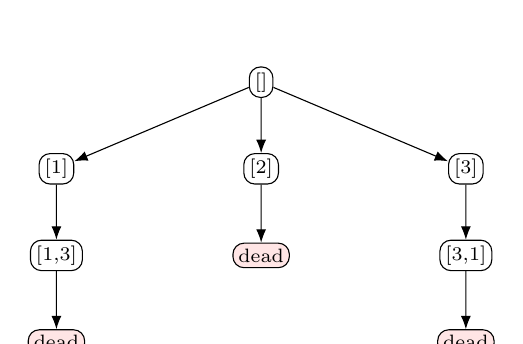
\begin{tikzpicture}[level distance=11mm,sibling distance=26mm,
  every node/.style={draw,rounded corners,inner sep=2pt,font=\scriptsize},
  edge from parent/.style={draw,-Latex}]
\node {[]} 
 child {node {[1]}
   child {node {[1,3]} child {node[fill=red!10] {dead}}}
 }
 child {node {[2]} child {node[fill=red!10] {dead}}}
 child {node {[3]}
   child {node {[3,1]} child {node[fill=red!10] {dead}}}
 };
\end{tikzpicture}
\end{center}

Explanation:
\begin{itemize}[leftmargin=6mm]
\item If row 1 uses column 1, row 2 can only safely use column 3; row 3 then has no safe column.
\item If row 1 uses column 2, row 2 has no safe column.
\item If row 1 uses column 3, the situation is symmetric to column 1.
\end{itemize}
Hence
\[
\boxed{\text{The 3-Queens problem has no solution.}}
\]
\end{answerbox}

% ---------------- Q5 ----------------
\section{Question 5 - Online Algorithms and Multithreading}

\begin{questionbox}{Q5(a) [4 marks]}
Find the worst-case competitive ratio of the second-chance page-replacement algorithm compared with the optimal page-replacement algorithm. The stated second-chance rule scans pages in FIFO order, gives an unmarked oldest page a second chance by moving/marking it, and removes an already marked oldest page.
\end{questionbox}

\begin{answerbox}
Let the cache contain \(k\) page frames. Second-chance is a deterministic demand-paging algorithm and is \emph{conservative}: on any request subsequence containing at most \(k\) distinct pages, it faults at most \(k\) times.

Partition a request sequence into phases, each containing at most \(k\) distinct pages. A conservative algorithm incurs at most \(k\) faults per phase. OPT must incur at least one fault for each new phase (up to an additive initial constant). Therefore
\[
\text{SC}(\sigma)\le k\,\text{OPT}(\sigma)+O(k).
\]
Thus second-chance is \(k\)-competitive.

The standard deterministic paging lower bound says no deterministic online paging algorithm with \(k\) frames can have competitive ratio smaller than \(k\) against an adversarial sequence. Hence the worst-case ratio is
\[
\boxed{k}.
\]
\end{answerbox}

\begin{questionbox}{Q5(b) [4 marks]}
Write a parallel algorithm to compute Fibonacci numbers. Specify the different threads and the interaction among them.
\end{questionbox}

\begin{answerbox}
A standard multithreaded recursive version uses one spawned thread for \(F_{n-1}\) while the current thread computes \(F_{n-2}\).

\begin{verbatim}
P-FIB(n)
    if n <= 1
        return n
    x = spawn P-FIB(n-1)   // child thread
    y =       P-FIB(n-2)   // current thread
    sync                     // wait for spawned child
    return x + y
\end{verbatim}

Thread interaction:
\[
\begin{array}{c}
P\text{-FIB}(n)\\
\swarrow\qquad\searrow\\
\text{spawn }P\text{-FIB}(n-1)\qquad P\text{-FIB}(n-2)\\
\multicolumn{1}{c}{\downarrow\ \text{sync}}\\
F_{n-1}+F_{n-2}=F_n
\end{array}
\]
The \texttt{sync} guarantees that both child computations finish before addition.
\end{answerbox}

\begin{questionbox}{Q5(c) [6 marks]}
Prove that the running time \(T_P\) of any multithreaded computation scheduled by a greedy scheduler on an ideal parallel computer with \(P\) processors is within a factor of 2 of an optimal scheduler.
\end{questionbox}

\begin{answerbox}
Let
\begin{itemize}[leftmargin=6mm]
\item \(T_1\) = total work,
\item \(T_\infty\) = span/critical-path length,
\item \(T_P^*\) = running time of an optimal scheduler on \(P\) processors.
\end{itemize}
Two universal lower bounds are
\[
T_P^*\ge \frac{T_1}{P},\qquad T_P^*\ge T_\infty.
\]
A greedy scheduler never leaves a processor idle when a ready strand exists. Its execution can be split into:
\begin{enumerate}[leftmargin=6mm]
\item \textbf{complete steps}, where all \(P\) processors work; their total time is at most \(T_1/P\),
\item \textbf{incomplete steps}, where fewer than \(P\) strands are ready; each such step advances the critical path, so their total is at most \(T_\infty\).
\end{enumerate}
Hence
\[
T_P\le \frac{T_1}{P}+T_\infty.
\]
Since both terms are at most \(T_P^*\),
\[
T_P\le 2T_P^*.
\]
Therefore a greedy scheduler is a 2-approximation to the optimal scheduler:
\[
\boxed{T_P\le2T_P^*}.
\]
\end{answerbox}

% ---------------- Q6 ----------------
\section{Question 6 - Reductions and NP-Completeness}

\begin{questionbox}{Q6(a) [2 marks]}
For a given problem, is it possible to find an optimal solution from a solution of a decision problem?
\end{questionbox}

\begin{answerbox}
For the standard optimization problems used in complexity theory, \textbf{yes}, when the optimization problem is self-reducible to its decision version.

First use the decision algorithm to determine the optimum objective value, often by binary search on a bound \(B\). Then reconstruct an optimal object by fixing one choice at a time and repeatedly asking whether a feasible solution with the optimum value still exists.

Thus polynomially many calls to the decision problem can recover an optimal solution whenever the usual polynomial self-reduction applies.
\end{answerbox}

\begin{questionbox}{Q6(b) [4 marks]}
Suppose \(Y\le_p X\). Justify:
\begin{enumerate}[label=(\roman*),leftmargin=7mm]
\item If \(X\) can be solved in polynomial time, then \(Y\) can be solved in polynomial time.
\item If \(Y\) cannot be solved in polynomial time, then \(X\) cannot be solved in polynomial time.
\end{enumerate}
\end{questionbox}

\begin{answerbox}
The notation \(Y\le_p X\) means there is a polynomial-time reduction from \(Y\) to \(X\).

\textbf{(i)} Given an instance of \(Y\), transform it to an instance of \(X\) in polynomial time and solve that instance using the polynomial-time algorithm for \(X\). Composition of polynomial-time procedures is polynomial, so \(Y\in P\).

\textbf{(ii)} This is the contrapositive of (i). If \(X\) were in \(P\), then (i) would force \(Y\in P\), contradicting the assumption. Therefore \(X\notin P\).
\end{answerbox}

\begin{questionbox}{Q6(c) [4 marks]}
Prove that the Traveling Salesman decision problem is NP-complete.
\end{questionbox}

\begin{answerbox}
Use the decision version:

\emph{Given a complete weighted graph and bound \(B\), is there a Hamiltonian tour of total cost at most \(B\)?}

\textbf{TSP is in NP.} A certificate is an ordering of the vertices. In polynomial time we check that every vertex appears exactly once and sum the tour weights to verify cost \(\le B\).

\textbf{TSP is NP-hard.} Reduce from Hamiltonian Cycle. Given an unweighted graph \(G=(V,E)\), build a complete graph \(G'\) on the same vertices with
\[
w(u,v)=\begin{cases}
1,&(u,v)\in E,\\
2,&(u,v)\notin E.
\end{cases}
\]
Set \(B=|V|\). A tour has cost at most \(|V|\) iff every edge of the tour has weight 1, which happens iff those edges form a Hamiltonian cycle in \(G\).

Thus
\[
HC\le_p TSP,
\]
so TSP is NP-hard. Since TSP is also in NP,
\[
\boxed{TSP\text{ is NP-complete}.}
\]
\end{answerbox}

\begin{questionbox}{Q6(d) [4 marks]}
Show that 3-CNF-SAT is reducible to the Clique problem.
\end{questionbox}

\begin{answerbox}
Let
\[
\phi=C_1\land C_2\land\cdots\land C_k
\]
be a 3-CNF formula.

Construct a graph as follows:
\begin{enumerate}[leftmargin=6mm]
\item Create one vertex for each literal occurrence in each clause.
\item Connect two vertices iff they come from \emph{different} clauses and their literals are not contradictory (not \(x\) and \(\neg x\)).
\item Ask whether the graph contains a clique of size \(k\).
\end{enumerate}

If \(\phi\) is satisfiable, choose one true literal from each clause. No two chosen literals contradict, so all chosen vertices are pairwise adjacent and form a \(k\)-clique.

Conversely, a \(k\)-clique can contain at most one vertex from each clause; because there are \(k\) clauses, it contains exactly one from each. Pairwise adjacency guarantees consistency, so the chosen literals can all be made true, satisfying every clause.

Therefore
\[
\boxed{3\text{-CNF-SAT}\le_p CLIQUE}.
\]
\end{answerbox}

% ---------------- Q7 ----------------
\section{Question 7 - RSA, Modular Equations, Extended Euclid}

\begin{questionbox}{Q7(a) [4 marks]}
RSA would be trivial to crack if the factorization of \(n\) into two primes were known in the public key. Explain why RSA would be trivial to crack knowing \(\phi(n)\).
\end{questionbox}

\begin{answerbox}
The public key is \((n,e)\), while the private exponent \(d\) satisfies
\[
ed\equiv1\pmod{\phi(n)}.
\]
If \(\phi(n)\) is known, compute
\[
\boxed{d=e^{-1}\bmod\phi(n)}
\]
with the extended Euclidean algorithm. Then ciphertext \(c\) is decrypted by
\[
\boxed{m\equiv c^d\pmod n}.
\]
Therefore knowing \(\phi(n)\) immediately reveals the private exponent. Likewise, if the factorization \(n=pq\) is known, then
\[
\phi(n)=(p-1)(q-1),
\]
so the same attack follows.
\end{answerbox}

\begin{questionbox}{Q7(b) [6 marks]}
How can we decide whether a modular equation
\[
ax\equiv b\pmod n
\]
is solvable? If a solution exists, how can we calculate it?
\end{questionbox}

\begin{answerbox}
Let
\[
d=\gcd(a,n).
\]
The congruence is solvable iff
\[
\boxed{d\mid b}.
\]

\textbf{Why?} The congruence means
\[
ax-b=qn
\]
for some integer \(q\), so \(b=ax-qn\) must be divisible by every common divisor of \(a\) and \(n\). Thus \(d\mid b\) is necessary; extended Euclid shows it is also sufficient.

If \(d\mid b\), divide by \(d\):
\[
a'=\frac ad,\quad b'=\frac bd,\quad n'=\frac nd.
\]
Now \(\gcd(a',n')=1\), so \(a'\) has an inverse modulo \(n'\). Compute it with EXTENDED-EUCLID and obtain
\[
x_0\equiv (a')^{-1}b'\pmod{n'}.
\]
There are exactly \(d\) incongruent solutions modulo \(n\):
\[
\boxed{x=x_0+k n',\qquad k=0,1,\ldots,d-1.}
\]
\end{answerbox}

\begin{questionbox}{Q7(c) [4 marks]}
What does \(\textsc{Extended-Euclid}(F_k,F_{k+1})\) return? Prove your answer.
\end{questionbox}

\begin{answerbox}
For the CLRS convention, \(\textsc{Extended-Euclid}(a,b)\) returns \((d,x,y)\) satisfying
\[
d=\gcd(a,b)=ax+by.
\]
Consecutive Fibonacci numbers are coprime, so \(d=1\). For \(k\ge2\), the returned coefficients are
\[
\boxed{
\textsc{Extended-Euclid}(F_k,F_{k+1})
=
\left(1,\;(-1)^kF_{k-1},\;(-1)^{k+1}F_{k-2}\right).
}
\]

Indeed, the Fibonacci identity
\[
F_kF_{k-1}-F_{k+1}F_{k-2}=(-1)^k
\]
gives
\[
F_k\bigl((-1)^kF_{k-1}\bigr)
+F_{k+1}\bigl((-1)^{k+1}F_{k-2}\bigr)=1.
\]
Also, Euclid's algorithm on consecutive Fibonacci numbers repeatedly uses
\[
F_{j+1}=F_j+F_{j-1},
\]
so after the initial quotient 0, all successive quotients are 1; back-substitution produces exactly the coefficients above.

Example, \(k=5\):
\[
\textsc{Extended-Euclid}(5,8)=(1,-3,2),
\]
because
\[
5(-3)+8(2)=1.
\]
\end{answerbox}

\newpage
\section*{Last-Minute Revision Sheet}
\addcontentsline{toc}{section}{Last-Minute Revision Sheet}

\begin{center}
\renewcommand{\arraystretch}{1.25}
\begin{tabularx}{\textwidth}{>{\bfseries}p{2cm} X}
\toprule
Topic & Must remember\\
\midrule
Double hashing & \(h(k,i)=(h_1(k)+ih_2(k))\bmod m\); Q1 table ends with slots \(0:22,2:59,3:17,4:4,5:15,6:28,7:88,9:31,10:10\).\\
Chaining & Successful expected search \(\Theta(1+\alpha)\).\\
Graham Scan & Sort by polar angle; pop while turn is non-left; hull = \((-10,4),(-9,-5),(6,-10),(8,-7),(8,6),(-7,8)\).\\
Kirkpatrick-Seidel & Output-sensitive \(O(n\lg h)\).\\
3 collinear & For each pivot sort slopes: \(O(n^2\lg n)\).\\
KMP & For \texttt{abbababbba}: \(\pi=[0,0,0,1,2,1,2,3,0,1]\).\\
Rabin-Karp & Pattern hash \(26\bmod11=4\); four verification windows: 15, 59, 92, 26.\\
3-Queens & No solution.\\
Second chance & Worst-case competitive ratio \(k\) for \(k\) frames.\\
Greedy scheduler & \(T_P\le T_1/P+T_\infty\le2T_P^*\).\\
Reduction & If \(Y\le_pX\) and \(X\in P\), then \(Y\in P\).\\
TSP NP-C & HC reduction with weights 1/2 and bound \(|V|\).\\
3SAT to Clique & One literal-occurrence vertex; connect compatible literals from different clauses; target clique size = number of clauses.\\
RSA & Knowing \(\phi(n)\) gives \(d=e^{-1}\bmod\phi(n)\).\\
Linear congruence & \(ax\equiv b\pmod n\) solvable iff \(\gcd(a,n)\mid b\).\\
Fib + EEA & \((1,(-1)^kF_{k-1},(-1)^{k+1}F_{k-2})\).\\
\bottomrule
\end{tabularx}
\end{center}

\end{document}
